\documentclass[11pt,a4paper]{article}
\usepackage[margin=2.3cm]{geometry}
\usepackage[T1]{fontenc}
\usepackage{lmodern,microtype}
\usepackage{amsmath,amssymb}
\usepackage{graphicx,booktabs,float,caption,array}
\usepackage[hidelinks]{hyperref}
\usepackage{xcolor}
\captionsetup{font=small,labelfont=bf}
\graphicspath{{../figures/}}
\setlength{\parskip}{4pt}
\newcommand{\done}{\textcolor{green!45!black}{\textbf{Completed}}}
\newcommand{\planned}{\textcolor{orange!80!black}{\textbf{Planned}}}

\title{\textbf{Game-Theoretic Social Compliance:\\ Teaching Autonomous Vehicles Human-Like Politeness and\\ Negotiation in Dense Urban Grids}\\[4pt]
\large Subjective--Objective Alignment, Social-Game-Theoretic Planning\\ and Operational Design Domain (ODD) Limits,\\ with results derived from a night-time Indian street dash-camera clip}
\author{Vishwas N.\\ M.Tech, Digital Electronics and Communication, MSRIT}
\date{\today}

\begin{document}
\maketitle

\begin{abstract}
Autonomous vehicles (AVs) in dense, mixed urban traffic often behave with machine-like rigidity or hesitation, because they optimise fixed safety/efficiency weights rather than reading the implicit social cues that human drivers use to share the road (inching forward, yielding gestures, patience). This report builds a small, fully reproducible pipeline around that gap. (i)~A classical computer-vision pass over a 249\,s night-time dash-camera clip of Indian streets extracts ego-motion, braking behaviour, tail-light-based headways and a crowding proxy. (ii)~Those video statistics parameterise a stylised multi-vehicle merge/crossing simulator with human-like opponents of latent courtesy. (iii)~Three planners are compared: a rigid gap-acceptance planner, an assertive planner, and a social game-theoretic planner with Bayesian type inference, an inching signal, a politeness cost and a safety shield. (iv)~Planners are scored with a five-dimension scorecard inspired by the Subjective--Objective Mapping Evaluation (SOME) framework (safety, comfort, efficiency, social interaction, impact on surrounding traffic).

In simulation the social planner reduces the ego delay from 16--20\,s to 4.5\,s and raises the weakest-link-aware score from 0.36--0.46 to 0.72, at the price of a small safety and comfort cost (0.5\% conflicts versus 0\%). The ablation study does \emph{not} show individual benefits for type inference, inching or the politeness term in this simulator, and the politeness sweep behaves counter-intuitively; these negative results are reported openly. All human-behaviour parameters in the simulator are assumed, not fitted, so the results demonstrate the method rather than validate it on real interactions.

(v)~A new ODD module asks how much of the real clip lies inside a structured, geofence-style ODD and how planners behave as conditions leave it. Under an illustrative specification only 6\% of the driving time (17\% without lane markings) is inside the ODD; a strict-ODD policy would start only about 25\% of trips under the clip's conditions, an ODD-unaware planner would have 5.0\% conflicts, and keeping short-term tracks of briefly missed vehicles halves conflicts (2.0\%) at 81\% availability, whereas simply inflating safety margins makes matters worse. These ODD results depend on assumed thresholds and an assumed perception-degradation model.
\end{abstract}

\section{Motivation and scope}
\subsection*{The core gap}
Conventional AV stacks are evaluated on binary outcomes (crash / no crash) and optimise fixed weights on safety and efficiency. In dense traffic with implicit negotiation, this yields two failure modes: \emph{over-hesitation} (waiting for a gap that never comes) and \emph{over-assertion} (taking gaps that force others to brake). Human drivers resolve such situations with subtle cues: inching forward to claim space, a polite wave, eye contact, or simply patience.

\subsection*{Evaluation: the SOME framework}
The Subjective--Objective Mapping Evaluation (SOME) framework, developed at Tongji University (corresponding author P.~Hang) and published in \emph{Communications in Transportation Research} (DOI 10.26599/COMMTR.2026.9640041), rates the ``intelligence'' of high-level AV behaviour rather than single functions such as braking. According to the public release~\cite{some}, it converts interaction data into structured text for a large language model that produces expert-style assessments, then trains an attention-based network to map ten objective metrics in five dimensions (safety, comfort, efficiency, social interaction, impact on surrounding traffic) to those assessments instead of using fixed manual weights. It was built on 5{,}200 interaction segments from the Waymo Open Dataset (following, merging, crossing) and tested on algorithms from six OnSite Challenge scenarios. The authors report that safety and comfort were most useful for separating intelligence levels, and that fixed-weight (AHP) aggregation can let strong safety mask weak comfort, efficiency or interaction. They list video and perception inputs as future work.

\textbf{What this report does and does not do.} It does \emph{not} reimplement the learned SOME model (no LLM annotation, no trained attention network, no Waymo data). It uses the same five \emph{dimensions} with nine hand-defined metrics, and reports two aggregates: an AHP-style fixed-weight mean and a weakest-link-aware weighted harmonic mean, to illustrate the masking effect the authors describe. Scores are therefore ``SOME-inspired'', not SOME scores.

\subsection*{ODD limits}
A second gap is the Operational Design Domain. Systems specified for mapped, structured, geofenced areas are expected to work inside them and to stop or hand over outside, which leaves dense, unstructured streets largely out of reach. Section~\ref{sec:odd} quantifies this on the clip and tests how the planner degrades.

\subsection*{Status summary}
\begin{center}\small
\begin{tabular}{@{}p{0.2\linewidth}p{0.72\linewidth}@{}}
\toprule
\done & Perception pass on the supplied video; video behaviour statistics; simulator parameterised from them; three planners and three ablations; five-dimension scorecard; politeness sweep; ODD conformance analysis of the clip and an ODD-degradation experiment with strict, unaware and adaptive policies; this report with all figures and tables.\\
\planned & Fitting the human-response model to real interaction trajectories; deep detector/tracker; camera calibration; learned SOME-style evaluator; integration into the earlier self-driving-car project; closing the safety gap (Section~\ref{sec:next}).\\
\bottomrule
\end{tabular}
\end{center}

\section{Video data and perception pipeline}
\subsection{Clip}
The supplied file is a 640$\times$360, 30\,fps, 248.8\,s night-time dash-camera recording of residential and commercial Indian streets (7{,}465 frames). Visual inspection shows the car parked at a gate for roughly the first 50\,s, then driving through streets with parked cars, two-wheelers, pedestrians, a stray dog and oncoming headlights.

\subsection{Method (classical CV only)}
No deep-learning detector was available offline in the workspace, so all perception is classical OpenCV on 15\,fps, 320$\times$180 frames, with CLAHE contrast enhancement and the bonnet (bottom 34\%) masked.
\begin{itemize}\setlength\itemsep{0pt}
\item \textbf{Ego speed proxy.} Two independent flow-based estimators from Farneb\"ack dense optical flow~\cite{farneback}: (a)~median ground-plane ratio $\Delta y/(y-y_h)^2$ over textured road pixels, and (b)~median radial expansion rate about the focus of expansion. They are put on a common scale and averaged, then smoothed (Gaussian, $\sigma\approx0.7$\,s). Their smoothed correlation is $r=0.85$. A third estimator (robust fit with a pitch offset) was tried and \emph{discarded} because it disagreed with the other two and produced negative speeds.
\item \textbf{Metric scale (assumed).} 70$^\circ$ horizontal field of view and 1.2\,m camera height. Speeds and accelerations are therefore approximate; they have no ground-truth check.
\item \textbf{Lead-vehicle range.} Pairs of red tail-light blobs on the same image row, assumed 1.5\,m apart, give range $Z=fW/w$ and time headway $Z/v$.
\item \textbf{Independent motion / crowding proxy.} Optical-flow residual after subtracting a radial ego-motion field; the fraction of pixels above threshold is the proxy.
\item \textbf{Lights and pedestrians.} Red and bright-white blob counts (tail- and head-lights) and an OpenCV HOG pedestrian detector.
\end{itemize}
Figure~\ref{fig:det} shows overlays. Tail-lights of a lead car are found (t=172\,s), but the independent-motion mask also lights up static buildings during turns and close passes (parallax), and the HOG detector fires rarely at night. \textbf{The crowding proxy is thus coarse and contaminated by parallax} and should be read as suggestive only.

\begin{figure}[H]\centering
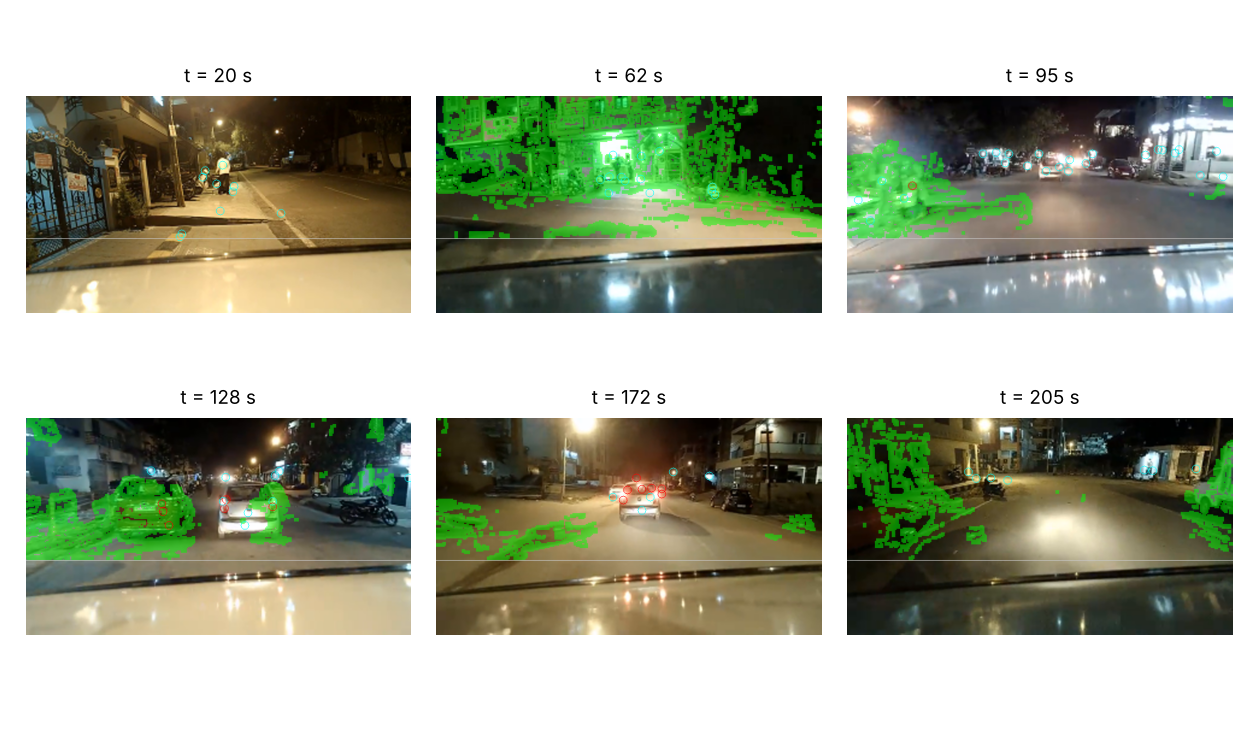
\includegraphics[width=\linewidth]{detections.png}
\caption{Perception overlays at six times: green = independent-motion residual, red circles = tail-light blobs, cyan circles = bright blobs, magenta = HOG pedestrian (none fired in these frames). Parallax contaminates the green mask on static structures.}\label{fig:det}
\end{figure}

\subsection{Video-derived results}
\begin{table}[H]\centering\small
\begin{tabular}{lr}\toprule
Quantity (approximate; see assumptions) & Value\\\midrule
Parked prefix before first motion & 49.1\,s\\
Mean speed while driving & 8.1\,m/s (29\,km/h)\\
90th-percentile speed & 12.5\,m/s\\
RMS acceleration / RMS jerk (driving, smoothed) & 1.76\,m/s$^2$ / 2.27\,m/s$^3$\\
5th / 95th percentile acceleration & $-2.73$ / $+2.96$\,m/s$^2$\\
Deceleration episodes ($a<-1$\,m/s$^2$, $\ge0.5$\,s) & 29\\
Frames with a lead tail-light pair detected & 8.8\%\\
Median lead range / median time headway / 10th pct headway & 10.3\,m / 1.45\,s / 0.84\,s\\
Mean red / white light blobs per frame & 1.2 / 15.8\\
Frames with a HOG pedestrian detection & 7.2\%\\\bottomrule
\end{tabular}\caption{Statistics extracted from the clip. Metric scale assumes 70$^\circ$ HFOV, 1.2\,m camera height and 1.5\,m lamp spacing.}\end{table}

Splitting the driving portion into terciles of the crowding proxy gives mean speeds of 6.3, 9.4 and 8.6\,m/s, RMS jerk of 1.5, 1.9 and 3.0\,m/s$^3$, and 5.5, 6.4 and 14.1 deceleration episodes per minute (sparse, medium, dense; Figure~\ref{fig:vdens}). The roughly 2.5$\times$ higher braking rate in the densest third agrees with the motivating picture of stop--go behaviour in crowded scenes, but it comes from a single clip and a contaminated proxy, so it is not a statistically tested finding. Speed and the crowding proxy are essentially uncorrelated ($r=0.04$).

\begin{figure}[H]\centering
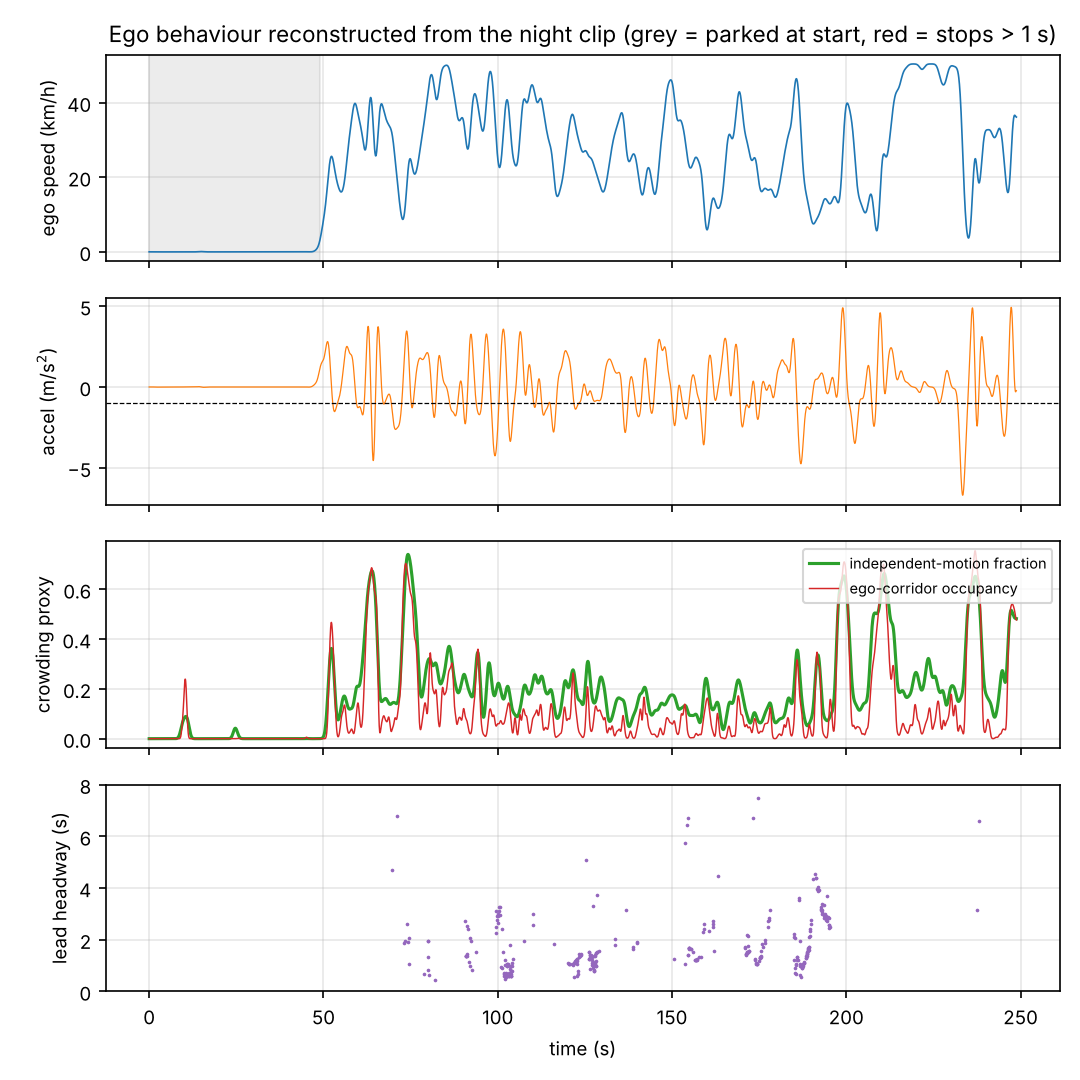
\includegraphics[width=\linewidth]{video_timeline.png}
\caption{Reconstructed ego behaviour: speed (grey = parked prefix), acceleration, crowding proxy and lead headway from tail-light pairs.}\label{fig:vtl}
\end{figure}
\begin{figure}[H]\centering
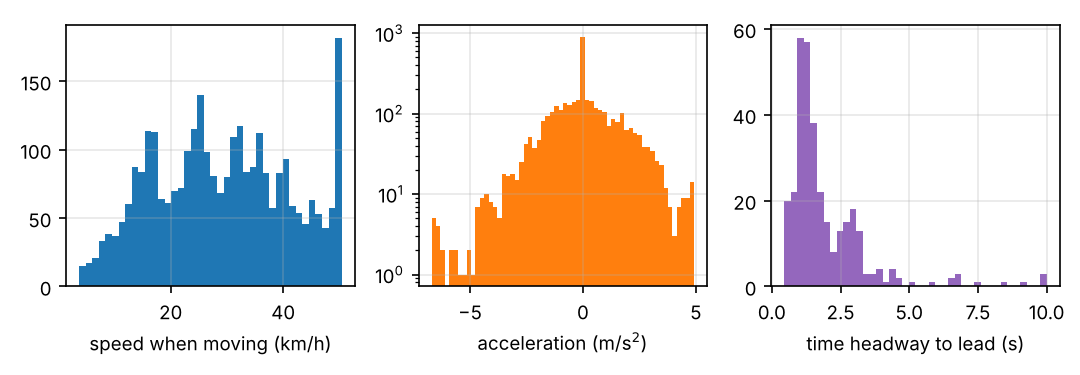
\includegraphics[width=\linewidth]{video_distributions.png}\\[2pt]
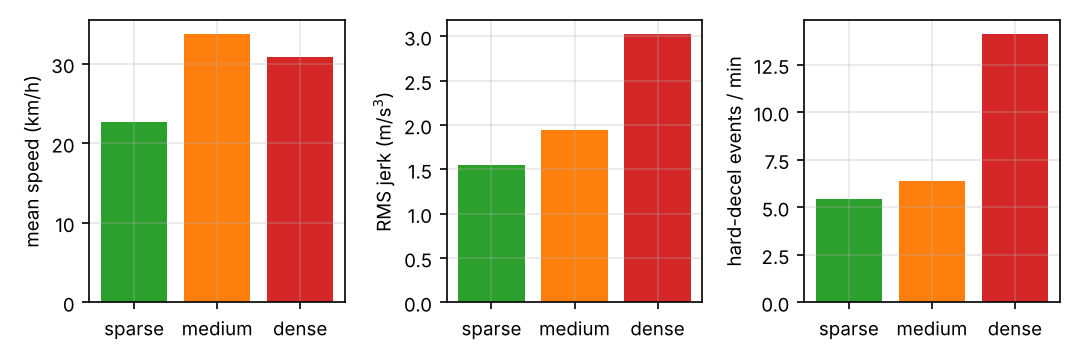
\includegraphics[width=\linewidth]{video_density.png}
\caption{Top: distributions of speed, acceleration and headway. Bottom: behaviour by crowding tercile.}\label{fig:vdens}
\end{figure}

\paragraph{Reliability.} Speed estimates before motion (0\,m/s in the parked prefix) and the plausible driving mean support the pipeline qualitatively, but there is no ground truth. The acceleration and jerk numbers are band-limited by smoothing and likely inflated by residual flow noise; they are used only as an order-of-magnitude comparison. A 2\%-quantile time-to-collision estimate from lamp ranges was computed but is not reported because it is dominated by range noise.

\section{Social game-theoretic planner}
\subsection{Scenario}
The ego vehicle approaches an unprotected conflict point (merge/crossing) and must pass a stream of $K=6$ human-like opponents. Each agent's front position $d$ is measured along its own path to the conflict point; the conflict zone is entered when $d>-1$\,m and left when the rear passes 1.5\,m. A conflict is counted when both occupy the zone at once. Post-encroachment time (PET) is the gap between one agent leaving and the other entering.

\subsection{Human opponent model (assumed)}
Each opponent has a latent courtesy type $\psi\in\{0,0.5,1\}$ (assertive, neutral, courteous; population prior 0.3/0.4/0.3). It observes the ego with a 0.5\,s delay and yields if
\begin{equation}
u_i<\sigma\!\big(\beta[\psi+\kappa\,c-\delta\,\rho-\theta]\big),
\end{equation}
where $u_i\sim U(0,1)$ is fixed per opponent, $\sigma$ is the logistic function, $c\in[0,1]$ is the ego's perceived \emph{claim} (larger when the ego is close to the zone and moving, i.e.\ inching or committing), $\rho$ is the opponent's urgency (time to the zone), and $(\beta,\theta,\kappa,\delta)=(6,0.7,0.8,0.6)$. This is a quantal-response-style choice~\cite{qre}. A yielding opponent decelerates to arrive after the ego clears (with a 1.25$\times$ safety factor), stops 0.6\,m short of the zone if needed, and gives up after a type-dependent patience (1.5/2.5/4\,s) while stopped. An emergency backstop (6\,m/s$^2$) applies if the ego is in the zone and the opponent is under 1.6\,s away. \textbf{These parameters were set by hand, not fitted to data.}

\subsection{Planners}
\begin{description}\setlength\itemsep{0pt}
\item[Rigid-safety.] Fixed gap-acceptance: go only if every opponent leaves a gap of at least 5\,s (constant-speed prediction); otherwise wait at the stop line. This represents machine-like hesitation.
\item[Assertive.] Same logic with a 1.5\,s gap threshold; no negotiation.
\item[Social (ours).] Each 0.2\,s the planner chooses among \emph{wait}, \emph{creep} (inch to 2\,m before the zone) and \emph{go} by minimising an expected cost:
\begin{align}
J_{\text{go}} &= T_{\text{clear}} + \lambda_s\,a_{\text{req}}^2,\qquad
J_{\text{wait}} = T_{\text{wait}}+2,\\
J_{\text{creep}} &= \sum_{\psi} b(\psi)\Big[p_\psi(c_{\text{creep}})\big(J_{\text{go}}+0.8\big)+\big(1-p_\psi(c_{\text{creep}})\big)\big(J_{\text{wait}}+0.6\big)\Big],
\end{align}
where $T_{\text{clear}}$ is the ego's time to clear the zone, $a_{\text{req}}$ is the deceleration the next opponent must apply to preserve a 0.8\,s margin (the politeness term, weight $\lambda_s=2$), $T_{\text{wait}}$ is the time until the first usable gap in the visible stream, and $p_\psi(c)$ is the predicted yield probability. The belief $b(\psi)$ is updated by Bayes' rule from whether the nearest opponent was observed to brake. The leader--follower structure is Stackelberg-like: the ego commits to a signal (inching) and anticipates the follower's response, in the spirit of~\cite{sadigh,schwarting}.
\item[Safety shield.] \emph{go} is permitted only if every live opponent is predicted (current acceleration; stopped yielders may restart after their remaining patience) to enter after $1.2\,T_{\text{clear}}+0.7$\,s or to have left $0.7$\,s before the ego could enter. Once the ego passes a point of no return (cannot stop before the zone at $3$\,m/s$^2$) it is committed.
\end{description}
Ablations remove type inference (belief fixed at the prior), the inching option, or the politeness term ($\lambda_s=0$). All planners share the same actuator limits (acceleration $-3$ to $+2$\,m/s$^2$, jerk limit 6\,m/s$^3$).

\subsection{Parameters taken from the video}
\begin{table}[H]\centering\small
\begin{tabular}{p{0.38\linewidth}p{0.52\linewidth}}\toprule
Simulator quantity & Source\\\midrule
Opponent free speeds (3--11\,m/s) & empirical driving-speed samples from the clip (clipped)\\
Inter-vehicle headways (0.8--10\,s) & empirical lead headways from tail-light pairs (clipped)\\
Density scaling of headways: 1.76 / 1.0 / 0.47 & ratio of mean crowding proxy across video terciles (sparse / medium / dense)\\
Ego approach speed & $0.6\times$ a video speed sample, clipped to 2--5\,m/s\\\midrule
Courtesy types, response parameters, patience, $K=6$ & \textbf{assumed} (not from the video)\\\bottomrule
\end{tabular}\caption{What is data-derived and what is assumed.}\end{table}

\subsection{Scorecard}
Nine metrics are mapped to $[0,1]$ with fixed thresholds and averaged per dimension: safety (no conflict; PET, full marks at $\ge2$\,s), comfort (RMS jerk; peak deceleration), efficiency (ego delay, zero at 25\,s), social interaction (unnecessary hesitation, i.e.\ stationary before the zone with no opponent within 3\,s; Jain fairness~\cite{jain} of delays across all agents), impact on others (mean induced deceleration, mean opponent delay). Overall scores: AHP-style $\sum_d w_d s_d$ with $w=(0.30,0.15,0.20,0.20,0.15)$ for (safety, comfort, efficiency, social, impact), and ``balanced'' $=1/\sum_d (w_d/s_d)$, which penalises a weak dimension.

\section{Results}
Each planner variant was run on 400 episodes per density (1{,}200 episodes), with identical seeds across planners (paired comparison). Confidence intervals are 95\% bootstrap (scores) or Wilson (proportions).

\begin{table}[H]\centering\footnotesize
\resizebox{\linewidth}{!}{\begin{tabular}{lrrrrrrr}
\toprule
Planner & Coll. \% [95\% CI] & Min PET (s) & Delay (s) & Stall (s) & RMS jerk & Induced dec. & Jain \\
\midrule
Rigid-safety & 0.0 [0.0,0.3] & 1.74 & 19.7 & 5.85 & 1.65 & 1.17 & 0.40 \\
Assertive & 0.0 [0.0,0.3] & 1.74 & 16.1 & 4.67 & 1.63 & 1.02 & 0.41 \\
Social game-theoretic (ours) & 0.5 [0.2,1.1] & 1.26 & 4.5 & 0.35 & 1.78 & 0.76 & 0.33 \\
\quad w/o type inference & 0.2 [0.0,0.6] & 1.26 & 4.5 & 0.26 & 1.65 & 0.68 & 0.32 \\
\quad w/o inching signal & 0.1 [0.0,0.5] & 1.38 & 4.4 & 0.65 & 1.55 & 0.86 & 0.34 \\
\quad w/o politeness term & 0.1 [0.0,0.5] & 1.26 & 4.3 & 0.30 & 1.75 & 0.73 & 0.33 \\
\bottomrule
\end{tabular}
}
\caption{Pooled results over all densities. PET = post-encroachment time; ``Induced dec.'' = mean deceleration of opponents beyond 0.8\,m/s$^2$; Jain = fairness of delays across ego and opponents (higher is more equal).}\end{table}

\begin{table}[H]\centering\footnotesize
\resizebox{\linewidth}{!}{\begin{tabular}{lrrrrrrr}
\toprule
Planner & Safety & Comfort & Efficiency & Social & Impact & AHP-style & Balanced \\
\midrule
Rigid-safety & 0.94 & 0.78 & 0.24 & 0.25 & 0.65 & 0.595 & 0.360 \\
Assertive & 0.93 & 0.78 & 0.37 & 0.32 & 0.70 & 0.640 & 0.460 \\
Social game-theoretic (ours) & 0.81 & 0.69 & 0.82 & 0.58 & 0.83 & 0.752 & 0.721 \\
\quad w/o type inference & 0.81 & 0.72 & 0.82 & 0.58 & 0.85 & 0.759 & 0.731 \\
\quad w/o inching signal & 0.84 & 0.80 & 0.82 & 0.56 & 0.82 & 0.774 & 0.737 \\
\quad w/o politeness term & 0.81 & 0.69 & 0.83 & 0.58 & 0.84 & 0.756 & 0.728 \\
\bottomrule
\end{tabular}
}
\caption{Five-dimension scorecard (mean over episodes).}\end{table}

\begin{figure}[H]\centering
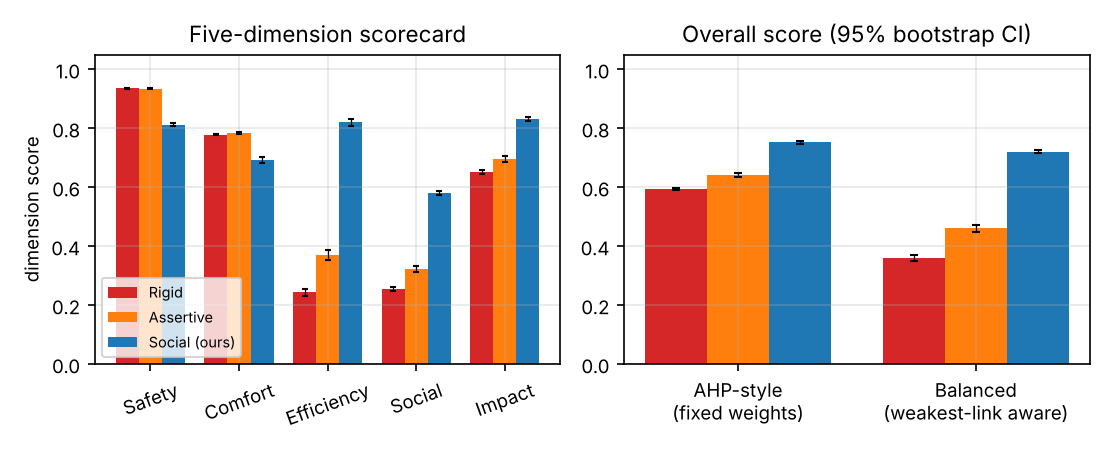
\includegraphics[width=\linewidth]{scorecard.png}
\caption{Dimension scores and overall scores with 95\% bootstrap intervals.}\label{fig:sc}
\end{figure}

\paragraph{Main effect.} Paired over identical scenarios, the social planner reduces ego delay by 15.2\,s [95\% CI 14.8--15.8] relative to the rigid planner and 11.6\,s [11.1--12.1] relative to the assertive planner. It also induces less deceleration in others ($-0.40$ and $-0.26$\,m/s$^2$ respectively). The AHP-style score rises by 0.157 and 0.112; the balanced score rises by 0.361 and 0.261. The rigid and assertive planners score $\approx0.94$ on safety but only 0.24--0.37 on efficiency and 0.25--0.32 on social interaction; the fixed-weight aggregate hides this (0.60--0.64) far more than the balanced one (0.36--0.46), consistent with the masking effect described for fixed-weight evaluation~\cite{some}.

\paragraph{Costs.} The social planner has 0.5\% conflicts (6 of 1{,}200; Wilson 95\% interval 0.2--1.1\%) versus none for the others, a lower mean minimum PET (1.26 vs.\ 1.74\,s), lower comfort (0.69 vs.\ 0.78), and \emph{lower} Jain fairness (0.33 vs.\ 0.40), because it equalises less: its own delay is small while some opponents wait. It is not yet at the safety level required of a deployable planner.

\begin{table}[H]\centering\footnotesize
\resizebox{0.95\linewidth}{!}{\begin{tabular}{llrrrrr}
\toprule
Density & Planner & Coll. \% & Delay (s) & Induced dec. & AHP & Balanced \\
\midrule
sparse & Rigid-safety & 0.0 & 23.8 & 1.13 & 0.569 & 0.232 \\
sparse & Assertive & 0.0 & 16.5 & 0.87 & 0.653 & 0.434 \\
sparse & Social game-theoretic (ours) & 0.0 & 2.6 & 0.52 & 0.795 & 0.766 \\
medium & Rigid-safety & 0.0 & 19.7 & 1.17 & 0.589 & 0.355 \\
medium & Assertive & 0.0 & 17.2 & 1.06 & 0.624 & 0.426 \\
medium & Social game-theoretic (ours) & 0.8 & 4.3 & 0.82 & 0.752 & 0.720 \\
dense & Rigid-safety & 0.0 & 15.8 & 1.20 & 0.625 & 0.492 \\
dense & Assertive & 0.0 & 14.7 & 1.13 & 0.643 & 0.520 \\
dense & Social game-theoretic (ours) & 0.8 & 6.6 & 0.95 & 0.709 & 0.677 \\
\bottomrule
\end{tabular}
}
\caption{Results by traffic density.}\end{table}
\begin{figure}[H]\centering
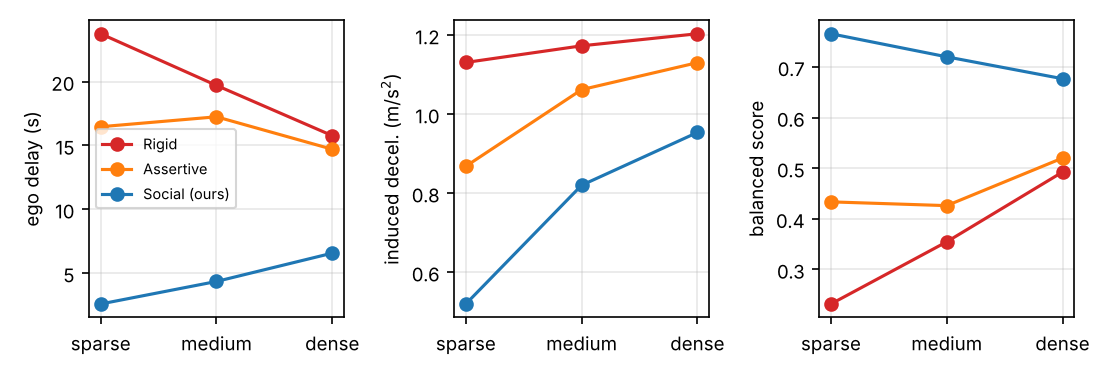
\includegraphics[width=\linewidth]{by_density.png}
\caption{Delay, induced deceleration and balanced score by density. The rigid planner's delay falls with density only because the fixed-length ($K=6$) stream finishes sooner when headways shrink; this is a simulator artefact, not evidence that denser traffic is easier.}
\end{figure}
\begin{figure}[H]\centering
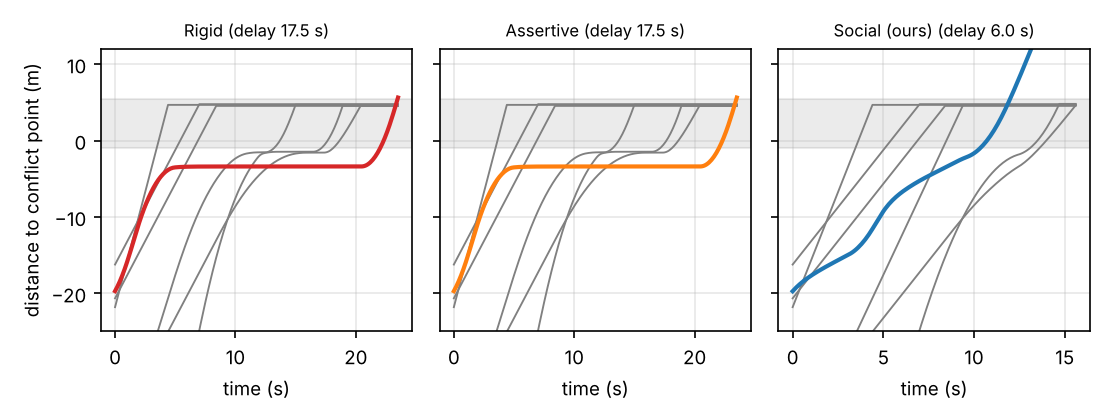
\includegraphics[width=\linewidth]{spacetime.png}
\caption{Space--time diagram for one dense scenario (seed 1002): grey = opponents, colour = ego, shaded band = conflict zone. The rigid and assertive egos wait at the line for the stream; the social ego slows, rolls up to the zone while opponents yield, and enters at about 10\,s.}
\end{figure}

\subsection{Ablations: a negative result}
\begin{figure}[H]\centering
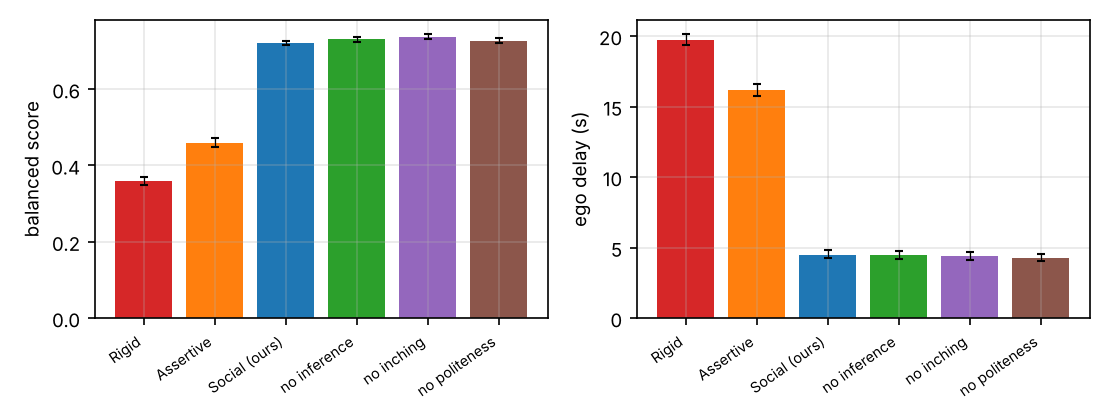
\includegraphics[width=\linewidth]{ablation.png}
\caption{Ablations (balanced score and ego delay, 95\% CI).}
\end{figure}
Removing type inference, the inching option or the politeness term does \emph{not} reduce the balanced score here (0.731, 0.737 and 0.728 versus 0.721 for the full planner). Ego delay is unchanged (4.3--4.5\,s). Removing inching slightly improves comfort and safety (0.1\% conflicts) and raises induced deceleration (0.86 vs.\ 0.76\,m/s$^2$) and hesitation (0.65 vs.\ 0.35\,s). In this simulator, therefore, the gain over the baselines comes from \emph{gap acceptance under a prediction-based shield together with courteous opponents who yield}, not from the individual game-theoretic components. The component claims in the concept paper are \textbf{not supported by these experiments}.

\subsection{Politeness sweep}
\begin{table}[H]\centering\footnotesize
\begin{tabular}{rrrrrr}
\toprule
$\lambda_s$ & Coll. \% & Delay (s) & Induced dec. & Opp. hard-brake \% & Balanced \\
\midrule
0 & 0.8 & 5.4 & 0.86 & 15.2 & 0.703 \\
0.5 & 0.8 & 5.4 & 0.88 & 16.0 & 0.702 \\
1 & 0.5 & 5.5 & 0.88 & 16.5 & 0.704 \\
2 & 0.8 & 5.8 & 0.88 & 19.0 & 0.696 \\
4 & 0.8 & 6.2 & 0.94 & 25.2 & 0.685 \\
8 & 1.0 & 6.8 & 0.95 & 29.8 & 0.670 \\
16 & 1.0 & 7.8 & 0.99 & 37.5 & 0.651 \\
\bottomrule
\end{tabular}

\caption{Social planner with varying politeness weight $\lambda_s$ (medium and dense density pooled, 400 episodes each; opponent hard-brake = any induced deceleration $>3$\,m/s$^2$ in an episode).}\end{table}
\begin{figure}[H]\centering
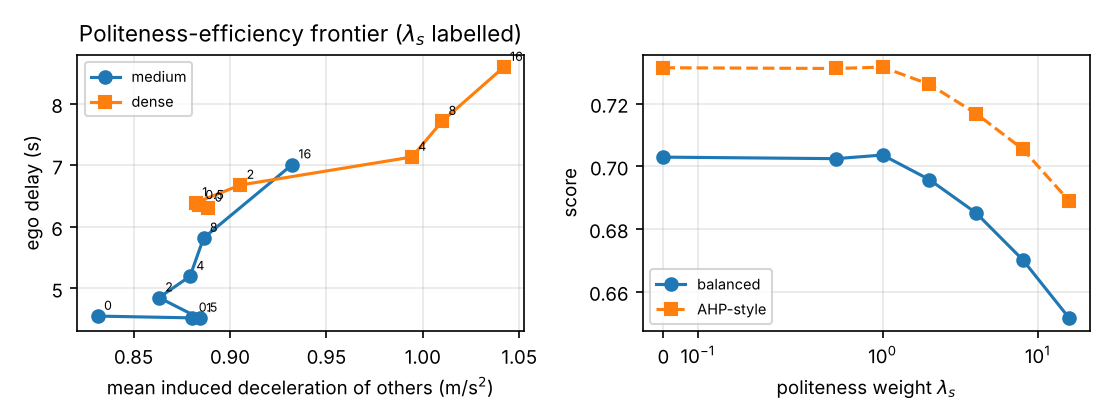
\includegraphics[width=\linewidth]{politeness_sweep.png}
\caption{Left: ego delay against induced deceleration across $\lambda_s$. Right: overall scores against $\lambda_s$.}
\end{figure}
Increasing $\lambda_s$ from 0 to 16 raises ego delay (5.4 to 7.8\,s) as intended, but induced deceleration \emph{rises} (0.86 to 0.99\,m/s$^2$) and opponent hard-braking episodes grow from 15\% to 38\%. A likely mechanism, not verified here, is that a more hesitant ego hovering near the line triggers courteous opponents to brake and stop for it, so the politeness term as implemented penalises the wrong event. The balanced score falls from 0.703 to 0.651. Treating this as a design flaw to fix, not as a tuning issue, is the first item of the next iteration.

\section{Operational Design Domain (ODD) limits}\label{sec:odd}
\subsection{Problem}
Most deployed autonomous driving systems are specified to work only inside an \emph{Operational Design Domain}: the operating conditions (road type, geography, lighting, weather, traffic) under which the system is designed to function~\cite{sae}. In practice this means strictly mapped, geofenced urban areas with structured roads, and the system is expected to hand over or stop when conditions leave that envelope (a ``minimal risk condition''). The concept paper's premise is that such systems work safely inside their mapped boundaries and fail outside them. We take that premise as the working hypothesis and do \emph{not} verify claims about any particular company's system. The questions studied here are quantitative:
\begin{enumerate}\setlength\itemsep{0pt}
\item How much of a real, dense, unstructured night-time Indian street drive would fall \emph{inside} a structured-urban ODD?
\item How does the social planner behave as conditions leave the ODD, and what are the options: refuse to operate (strict ODD), carry on unaware, or adapt?
\end{enumerate}

\subsection{ODD specification and runtime monitor}
We define an illustrative ODD with five attributes, each measured per frame from the clip by a classical-CV proxy (Table~\ref{tab:oddspec}). The thresholds are \emph{assumed} (they stand for a structured, lit, marked-lane, moderate-traffic domain) and are varied in a sensitivity analysis. Each attribute has a quality $q_k\in[0,1]$ ($1$ when inside the specification, falling linearly to $0$ at twice the threshold excursion), smoothed over about 1\,s. The \emph{ODD monitor} outputs $q=\min_k q_k$ (weakest link). Two variants are used: $q_{\text{all}}$ over all five attributes (strict ODD) and $q_{\text{perc}}$ over the four attributes that matter for detecting other road users (lane markings excluded).

\begin{table}[H]\centering\small
\begin{tabular}{p{0.2\linewidth}p{0.5\linewidth}p{0.2\linewidth}}\toprule
Attribute & Video proxy & Inside if\\\midrule
Lane markings & total length of near-diagonal Hough lines in the road region, as a fraction of image width & $\ge 0.15$\\
Lighting & fraction of road-region pixels with luma $<30$ & $\le 0.12$\\
Glare & fraction of road-region pixels saturated ($\ge250$) & $\le 0.02$\\
Traffic complexity & independent-motion fraction (Section~2) & $\le 0.15$\\
Image sharpness & variance of the Laplacian of the road region & $\ge 800$\\\bottomrule
\end{tabular}\caption{Illustrative ODD attributes (thresholds assumed).}\label{tab:oddspec}\end{table}

\subsection{How much of the clip is inside the ODD?}
Over the 199.7\,s of driving, \textbf{only 6.1\% of the time satisfies all five attributes}, and 17.2\% satisfies the four attributes other than lane markings. After a 1\,s debounce the status exits the ODD 2.4 times per minute, and the mean uninterrupted time inside is about 1\,s, so a strict ODD would be unusable rather than merely often violated. The attributes violated most are lane markings (74\% of driving time) and traffic complexity (64\%), followed by lighting (23\%), sharpness (19\%) and glare (15\%) (Figures~\ref{fig:oddframes}--\ref{fig:oddviol}).

\begin{figure}[H]\centering
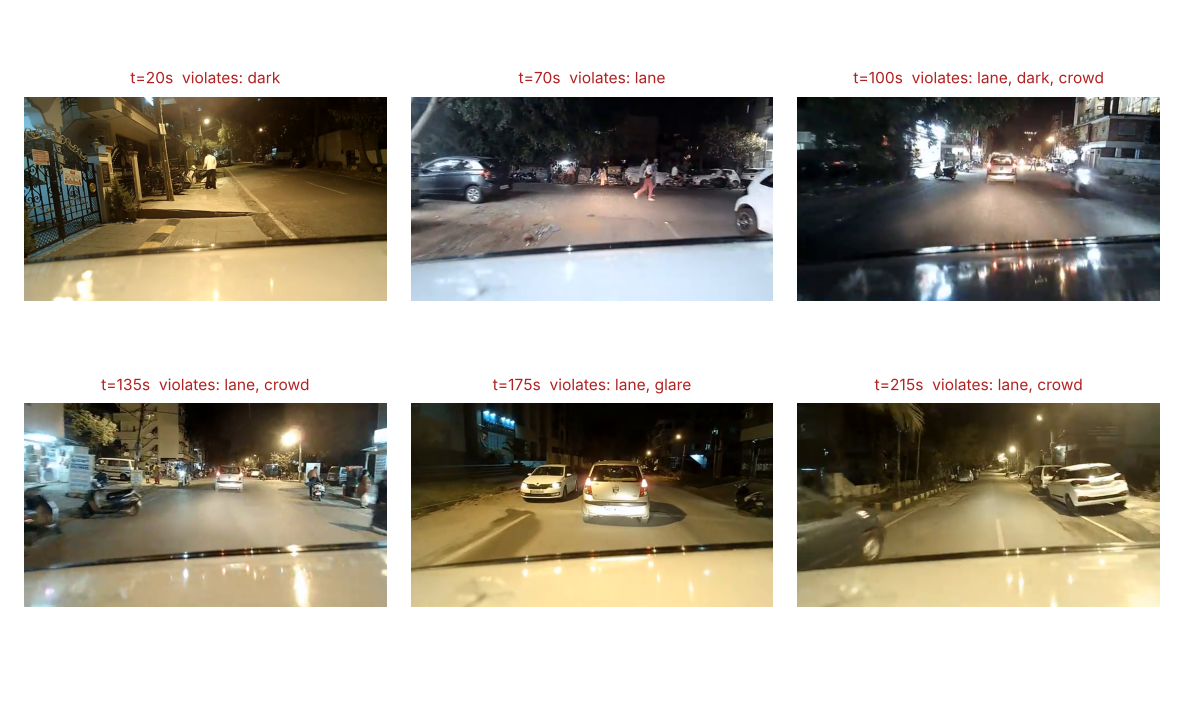
\includegraphics[width=\linewidth]{odd_frames.png}
\caption{Six frames labelled with the ODD attributes they violate. Note t=215\,s: dashed lane markings are visible but the lane proxy flags a violation (see caveat below).}\label{fig:oddframes}
\end{figure}
\begin{figure}[H]\centering
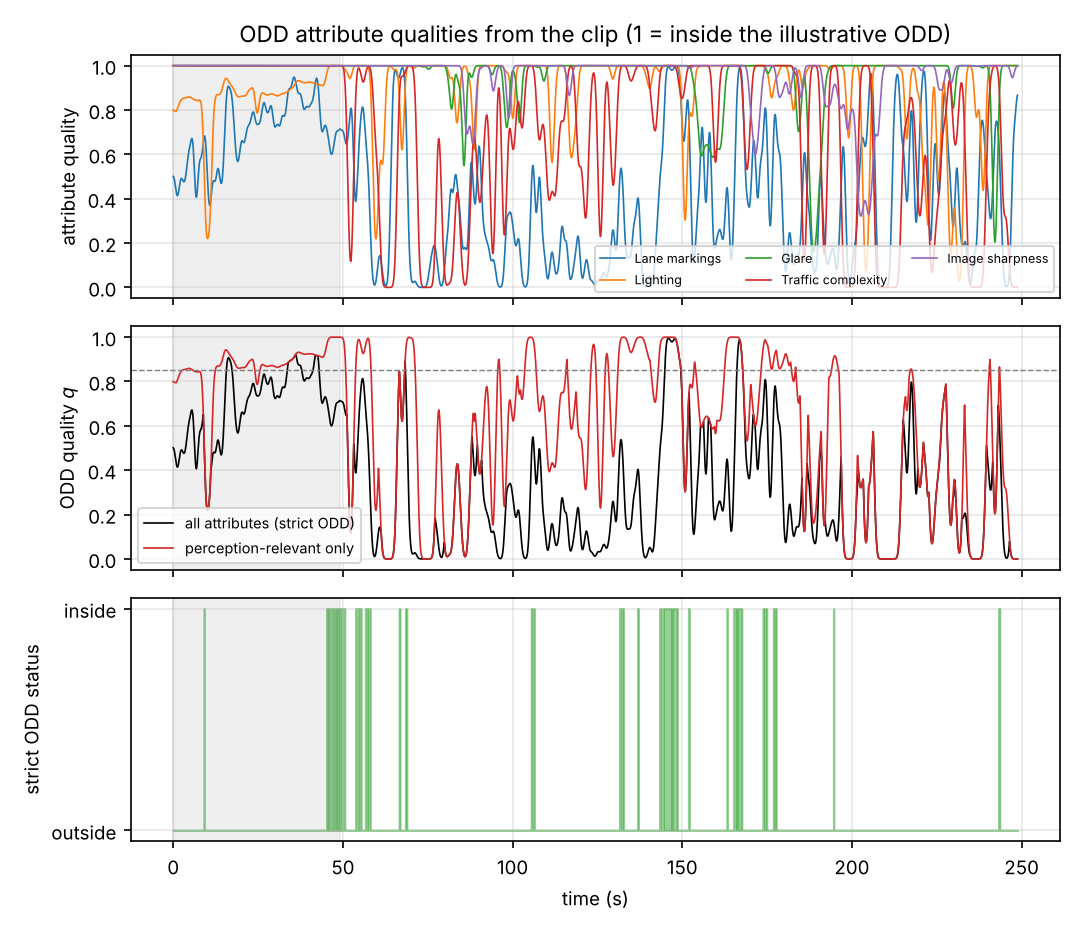
\includegraphics[width=\linewidth]{odd_timeline.png}
\caption{Attribute qualities, monitor output $q$ and strict ODD status through the clip (grey = parked prefix). The dashed line marks $q=0.85$, the strict-ODD disengagement threshold used later.}\label{fig:oddtl}
\end{figure}
\begin{figure}[H]\centering
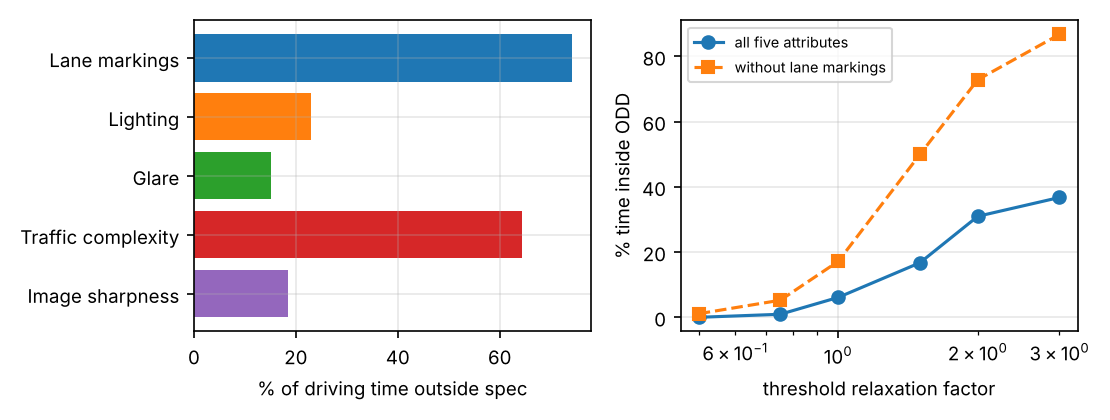
\includegraphics[width=\linewidth]{odd_violations.png}
\caption{Left: share of driving time each attribute is outside its specification. Right: time inside the ODD as all thresholds are relaxed by a common factor (log scale).}\label{fig:oddviol}
\end{figure}

\begin{table}[H]\centering\small
\begin{tabular}{lrrrrrr}\toprule
Threshold relaxation factor & 0.5 & 0.75 & 1 & 1.5 & 2 & 3\\\midrule
Inside ODD, all five attributes (\%) & 0.0 & 0.9 & 6.1 & 16.7 & 31.0 & 36.7\\
Inside ODD, without lane markings (\%) & 1.1 & 5.2 & 17.2 & 49.9 & 72.9 & 86.7\\\bottomrule
\end{tabular}\caption{Sensitivity of ODD conformance to the assumed thresholds.}\end{table}

\paragraph{Descriptive comparison with the human driver.} In the 6\% of time inside the ODD the human driver averaged 7.1\,m/s with RMS jerk 1.79\,m/s$^3$; outside, 8.2\,m/s and 2.30\,m/s$^3$. With so little time inside, this is a description, not evidence that conditions outside the ODD change driver behaviour.

\paragraph{Caveat: the proxies lean towards violation.} The lane proxy misses dashed markings that are visible in the frames (t=215\,s in Figure~\ref{fig:oddframes}), and the traffic-complexity proxy is inflated by parallax from near structures (Section~2). The 6\% figure should therefore be read as a lower bound. However, relaxing every threshold by a factor of two still leaves the full ODD satisfied for only 31\% of the time (73\% without lane markings), so the qualitative conclusion, that this environment is mostly outside a structured ODD, is robust to the proxy choice.

\subsection{Planner behaviour as conditions leave the ODD}
\paragraph{Degradation model (assumed).} We let a scene-level ODD quality $q$ degrade the ego's perception of opponents: position noise $\sigma_d=0.3+3(1-q)$\,m, speed noise $\sigma_v=0.1+(1-q)$\,m/s, per-step miss probability $0.35(1-q)^2$ and latency $0.5(1-q)$\,s. The monitor observes $\hat q=q+\mathcal N(0,0.05^2)$. This mapping is not fitted to any sensor.

\paragraph{Policies.}
\begin{description}\setlength\itemsep{0pt}
\item[Strict-ODD (geofence-style).] Runs the social planner if $\hat q\ge0.85$, otherwise disengages (no trip). We assume the resulting minimal-risk stop is perfectly safe, which favours this policy on safety.
\item[ODD-unaware.] Runs the social planner at any $q$.
\item[ODD-aware: persistence.] Keeps a track of a briefly undetected opponent for up to 1.5\,s, extrapolating at constant velocity; disengages only if $\hat q<0.15$.
\item[ODD-aware: persistence + margins.] Additionally inflates the safety-shield margins by $1+1.5(1-\hat q)$.
\end{description}
Experiments use the medium-density scenario. A controlled sweep covers $q\in\{1.0,0.9,\dots,0.1\}$ (300 episodes per point and policy). A video-conditioned run draws $q$ from the empirical distribution of $q_{\text{perc}}$ over the driving portion of the clip (median 0.61, quartiles 0.26 and 0.85) with 900 episodes per policy.

\begin{figure}[H]\centering
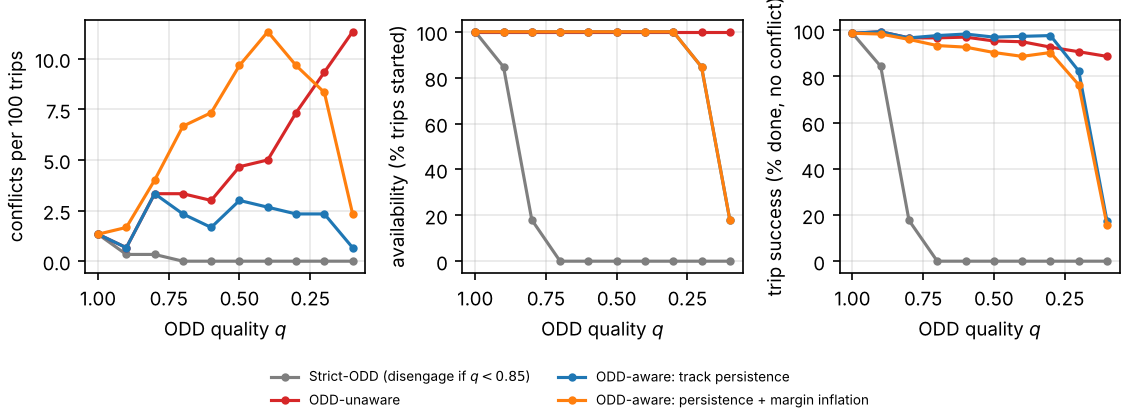
\includegraphics[width=\linewidth]{odd_sweep.png}
\caption{Conflicts, availability and trip success against ODD quality $q$ (note the reversed axis). Points are noisy (300 episodes each).}\label{fig:oddsweep}
\end{figure}

\begin{table}[H]\centering\footnotesize
\resizebox{\linewidth}{!}{\begin{tabular}{lrrrrr}
\toprule
Policy & Avail. \% & Coll. \% (of all) & Coll. \% (if started) & Success \% & Delay (s) \\
\midrule
Strict-ODD (geofence-style) & 25.3 & 0.33 & 1.32 & 25.0 & 4.4 \\
ODD-unaware & 100.0 & 5.00 & 5.00 & 95.0 & 3.6 \\
ODD-aware: persistence & 81.0 & 2.00 & 2.47 & 79.0 & 4.7 \\
ODD-aware: persistence + margins & 81.6 & 4.44 & 5.45 & 77.1 & 11.5 \\
\bottomrule
\end{tabular}
}
\caption{Video-conditioned results ($q$ sampled from the clip's $q_{\text{perc}}$ distribution, 900 episodes per policy). ``Avail.'' = trips started; ``Success'' = trips completed without conflict; delay is over started trips.}\label{tab:oddvideo}\end{table}

\paragraph{Findings.}
\begin{itemize}\setlength\itemsep{1pt}
\item \textbf{The ODD is the binding constraint.} With conditions like the clip's, the strict-ODD policy would start only 25\% of trips; below $q=0.85$ it starts none (Figure~\ref{fig:oddsweep}, middle). Its safety is excellent (0.3\% conflicts over all trips), but this partly reflects trips that never happen.
\item \textbf{Operating unaware is unsafe, and increasingly so.} Conflicts rise from 1.3\% at $q=1$ to 11\% at $q=0.1$; under the clip's conditions the unaware planner has 5.0\% conflicts.
\item \textbf{Cheap robustness helps.} Track persistence keeps conflicts at roughly 1--3\% across $q$ from 0.2 to 0.9 and cuts the video-conditioned conflict rate from 5.0\% to 2.0\% (2.5\% of started trips) at 81\% availability and a small delay increase (4.7\,s versus 3.6\,s unaware).
\item \textbf{Being more conservative can backfire.} Adding margin inflation raised delay to 11.5\,s and conflicts to 4.4\% (5.5\% of started trips), worse than persistence alone and, at mid $q$, worse than doing nothing (up to 11\% around $q=0.4$). In an isolation test at $q=0.8$ and $0.5$, margin inflation without persistence gave 5.7\% and 18.7\% conflicts. A plausible mechanism, not verified here, is that longer waits give courteous opponents time to stop, lose patience and restart, which lengthens exposure; it echoes the hesitation effect seen in the politeness sweep.
\end{itemize}
Together these results support a graded view of the ODD (strict boundary, degraded-but-monitored operation, minimal-risk fallback) over a hard geofence, but only under the assumed degradation model; they do not show that any particular adaptation would work on a real vehicle.


\section{Discussion and limitations}
\begin{itemize}\setlength\itemsep{1pt}
\item \textbf{Simulation, not validation.} The human model, its parameters and the stream length are assumed; the planner knows the functional form of the human model, which favours it. The numbers show the framework working end to end, not performance on real roads.
\item \textbf{Video link is thin.} The clip supplies speed/headway distributions and a density scaling, not interaction trajectories. Perception is classical, uncalibrated and unvalidated against ground truth; the crowding proxy is contaminated by parallax.
\item \textbf{Scorecard.} Thresholds and weights are hand-chosen; changing them changes absolute values (not shown here). It is not the learned SOME model.
\item \textbf{Safety.} 0.5\% conflicts is not acceptable for deployment; failures arise from yielders that lose patience or from prediction mismatch during the commit phase.
\item \textbf{ODD analysis.} Thresholds are illustrative; the lane and traffic-complexity proxies lean towards violation; the perception-degradation model and the ``safe minimal-risk stop'' assumption are not grounded in real sensor or vehicle data; no real AV failure data were used.
\item \textbf{Fairness metric.} Jain fairness of delays favours equal suffering; it may not be the right notion of right-of-way sharing.
\end{itemize}

\section{Next iteration}\label{sec:next}
\begin{enumerate}\setlength\itemsep{1pt}
\item Redesign the politeness cost to include \emph{hesitation-induced} braking (penalise ego dwell time near the line while others yield) and re-run the sweep.
\item Tighten the shield (patience-aware restart predictions, wider commit margins) targeting 0 conflicts in $\ge10^4$ episodes.
\item Make type inference informative (observe opponent acceleration profiles rather than a yield/hold bit) and test where it matters, e.g.\ mixed fleets with a higher share of assertive drivers.
\item Fit the human-response model to real interaction trajectories (e.g.\ merging/crossing datasets) and re-evaluate; compare against the scorecard of a learned SOME-style evaluator.
\item Replace classical perception with a deep detector and tracker, calibrate the camera, and extract real interaction events from additional clips.
\item Ground the ODD module: calibrate the ODD thresholds and the $q\to$ perception-degradation mapping on real sensor logs, replace the lane and complexity proxies with learned detectors, and add a graceful-degradation policy (speed and manoeuvre restriction, remote assistance) alongside the minimal-risk stop.
\item Integrate the planner and scorecard into the earlier self-driving-car simulation project.
\end{enumerate}

\section{Reproducibility}
Code is in \texttt{code/}: \texttt{perception.py} (per-frame perception), \texttt{video\_analysis.py} (statistics and video figures), \texttt{socialsim.py} (simulator and planners), \texttt{evaluate.py} (episodes, scorecard, tables and figures), \texttt{viz\_detections.py} (overlay figure), \texttt{odd\_features.py} and \texttt{odd\_experiment.py} (ODD attributes, conformance analysis, ODD-degradation experiment). \texttt{run\_all.sh} runs everything; \texttt{report/} builds with \texttt{pdflatex main.tex}. Dependencies: Python 3 with OpenCV, NumPy, SciPy, pandas, Matplotlib. Raw outputs are in \texttt{data/}.

\begin{thebibliography}{9}\small
\bibitem{some} Tongji University team (corresponding author P.~Hang), ``Subjective--Objective Mapping Evaluation (SOME) of intelligence in autonomous driving,'' \emph{Communications in Transportation Research}, DOI 10.26599/COMMTR.2026.9640041; summarised in the public release at \url{https://www.eurekalert.org/news-releases/1150789}. Read via the press release only; the original article was not accessed.
\bibitem{sae} SAE International, \emph{J3016: Taxonomy and Definitions for Terms Related to Driving Automation Systems for On-Road Motor Vehicles}, 2021 (definition of ODD and minimal risk condition). See also ISO 34503:2023 on ODD taxonomy.
\bibitem{farneback} G.~Farneb\"ack, ``Two-frame motion estimation based on polynomial expansion,'' \emph{SCIA}, 2003.
\bibitem{qre} R.~McKelvey and T.~Palfrey, ``Quantal response equilibria for normal form games,'' \emph{Games and Economic Behavior}, 1995.
\bibitem{sadigh} D.~Sadigh, S.~Sastry, S.~Seshia, A.~Dragan, ``Planning for autonomous cars that leverage effects on human actions,'' \emph{RSS}, 2016.
\bibitem{schwarting} W.~Schwarting, A.~Pierson, J.~Alonso-Mora, S.~Karaman, D.~Rus, ``Social behavior for autonomous vehicles,'' \emph{PNAS}, 2019.
\bibitem{jain} R.~Jain, D.~Chiu, W.~Hawe, ``A quantitative measure of fairness and discrimination for resource allocation in shared computer systems,'' DEC-TR-301, 1984.
\end{thebibliography}
\end{document}
